\documentclass[12pt]{article}

\usepackage[spanish]{babel}
\usepackage[none]{hyphenat}
\usepackage[left=1.5cm, right=1.5cm, top = 2cm, bottom=2.5cm]{geometry}
\usepackage{parskip}
\usepackage[export]{adjustbox}
\usepackage{enumitem}[shortlabels]
\usepackage{listings} 
\usepackage{color}
\usepackage{fancyhdr}
\usepackage{graphicx}
\usepackage{caption} 
% \usepackage{subcaption}
\usepackage{wrapfig}
% \usepackage{longtable}
% \usepackage{multirow, makecell}
% \usepackage{amsmath} 
\usepackage[hidelinks]{hyperref}
\usepackage{csquotes}
% \usepackage{tocloft}

\newcommand{\linejump}{\hfill \break}
\renewcommand{\thefootnote}{\fnsymbol{footnote}}
% \newcommand{\unit}[1]{\ensuremath{\, \mathrm{#1}}}

\definecolor{dkgreen}{rgb}{0,0.6,0}
\definecolor{gray}{rgb}{0.5,0.5,0.5}
\definecolor{mauve}{rgb}{0.58,0,0.82}
\lstset{
  language=Java,
  aboveskip=3mm,
  belowskip=3mm,
  showstringspaces=false,
  columns=flexible,
  basicstyle={\scriptsize\ttfamily},
  numbers=none,
  numberstyle=\tiny\color{gray},
  keywordstyle=\color{blue},
  commentstyle=\color{dkgreen},
  stringstyle=\color{mauve},
  breaklines=true,
  breakatwhitespace=true,
  tabsize=2
}

\sloppy
\setlength{\parindent}{0cm}
\setlength{\columnsep}{0.5cm}
\decimalpoint
\graphicspath{{img/}}

\hypersetup{colorlinks=true, urlcolor=blue, citecolor=blue}
\urlstyle{same}

\pagestyle{fancyplain}
\fancyhf{}
\fancyhead[L]{\scriptsize 
  Universidad Nacional Autónoma de México \\
  Programación Orientada a Objetos \\
  M.C. Leonardo Ledesma Dominguez
}
\fancyhead[R]{\thepage}


\begin{document}
  \begin{center}
    Acosta Porcayo Alan Omar, Gutiérrez Grimaldo Alejandro, Medina Villa Samuel

    \linejump
    \LARGE \textbf{Tarea 8. Manejo de archivos y seralización}
  \end{center}
  
  \linejump
  \begin{enumerate}
    \item Estudie el programa que se vio en clase ubicado en: \url{https://github.com/LeonardoLed/POO/blob/main/TemaVI.ManejoArchivos/Principal.java}
    
    Modifique al programa para aumentar la funcionalidad de dicho programa, para que realice:
    \begin{enumerate}[label=\alph*)]
      \item Solicite de manera separada nombre, apellido paterno, apellido materno y edad que se escriba en un archivo datos.txt.
      \item Ocupe serialización/deserialización para reconstruir los objetos creados anteriormente que provengan del archivo datos.txt
    \end{enumerate}

    \textit{\textbf{Principal.java}}
    \begin{lstlisting}
import java.io.*;
import javax.swing.JOptionPane;

class Persona implements Serializable {
  String nombre;
  String apellidoPaterno;
  String apellidoMaterno;
  int edad;

  public Persona(String nombre, String apellidoPaterno, String apellidoMaterno, int edad) {
    this.nombre = nombre;
    this.apellidoPaterno = apellidoPaterno;
    this.apellidoMaterno = apellidoMaterno;
    this.edad = edad;
  }
}

public class Principal {
  public static void main(String[] args) {
    File archivo = new File("datos.txt");

    String nombre = JOptionPane.showInputDialog(null, "Escribe tu nombre");
    String apellidoPaterno = JOptionPane.showInputDialog(null, "Escribe tu apellido paterno");
    String apellidoMaterno = JOptionPane.showInputDialog(null, "Escribe tu apellido materno");
    int edad = Integer.parseInt(JOptionPane.showInputDialog(null, "Escribe tu edad"));

    Persona persona = new Persona(nombre, apellidoPaterno, apellidoMaterno, edad);

    try {
      if (!archivo.exists()) {
        archivo.createNewFile();
      }

      ObjectOutputStream oos = new ObjectOutputStream(new FileOutputStream(archivo));
      oos.writeObject(persona);
      oos.close();

      ObjectInputStream ois = new ObjectInputStream(new FileInputStream(archivo));
      Persona personaLeida = (Persona) ois.readObject();
      ois.close();

      System.out.println("Nombre: " + personaLeida.nombre);
      System.out.println("Apellido Paterno: " + personaLeida.apellidoPaterno);
      System.out.println("Apellido Materno: " + personaLeida.apellidoMaterno);
      System.out.println("Edad: " + personaLeida.edad);
    } catch (IOException | ClassNotFoundException e) {
      e.printStackTrace();
    }
  }
}
    \end{lstlisting}

    \textbf{Ejecución}
    \begin{figure}[h!]
      \centering
      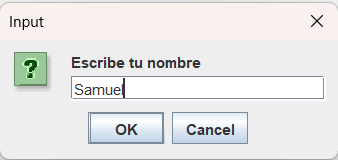
\includegraphics[width=0.4\textwidth]{P1A.png}
    \end{figure}
    \begin{figure}[h!]
      \centering
      
\includegraphics[width=0.4\textwidth]{P1B.png}
      
    \end{figure}

    \item Modifique el programa de Snake realizado en la práctica 4 para que guarde en un archivo los llamados High Scores imprimiendo en un archivo hs.txt el nombre del usuario y puntos obtenidos.
    
    Considere la diferencia de puntuación según el nivel de juego:
    \begin{enumerate}[label=\alph*.]
      \item Babosa 1 pt.
      \item Gusano 1.5 pt.
      \item Anaconda 2 pts.
    \end{enumerate}

    \textit{\textbf{HighScores.java}}
    \begin{lstlisting}
import java.io.File;
import java.io.IOException;
import java.io.PrintWriter;

import java.util.Scanner;
import java.util.StringTokenizer;
import java.util.HashMap;

public class HighScores {
  private static final int MAX_SCORES = 10;
  private static HashMap<String, Double> scores = new HashMap<>();

  public static boolean canInsert(double score) {
    scores.clear();
    try (Scanner reader = new Scanner(new File("hs.txt"))) {
      while (reader.hasNextLine() && scores.size() < MAX_SCORES) {
        String line = reader.nextLine();
        StringTokenizer tokenizer = new StringTokenizer(line, " - ");
        scores.put(tokenizer.nextToken(), Double.parseDouble(tokenizer.nextToken()));
      }
    } catch (IOException e) {}

    if (scores.size() < MAX_SCORES) {
      return true;
    } else {
      double minScore = 999999999;
      String minName = "";
      for (String key : scores.keySet()) {
        if (scores.get(key) < minScore) {
          minScore = scores.get(key);
          minName = key;
        }
      }
      if (score > minScore) {
        scores.remove(minName);
        return true;
      }
    }
    return false;
  }

  public static void insert(String name, double score) {
    scores.put(name, score);
  }

  public static void save() {
    try (PrintWriter writer = new PrintWriter("hs.txt")) {
        for (String key : scores.keySet()) {
            writer.println(key + " - " + scores.get(key));
        }
    } catch (IOException e) {
        System.out.println("Error al guardar los puntajes");
    }
  }
}
    \end{lstlisting}

    \textbf{Modificación en \textit{Board.java}}
    \begin{lstlisting}
private void gameOver(Graphics g) {
  timer.stop();

  if (HighScores.canInsert(score)) {
    String name = JOptionPane.showInputDialog(
      this,
      "Ingresa tu nombre",
      "Nuevo Record",
      JOptionPane.QUESTION_MESSAGE);

    HighScores.insert(name, score);
    HighScores.save();
  }

  int n = JOptionPane.showConfirmDialog(
    this,
    "Quieres volver a jugar?",
    "Game Over",
    JOptionPane.YES_NO_OPTION);
      
  if (n == JOptionPane.YES_OPTION) {
    inGame = true;
    score = 0;
    initGame();
  } else {
    JOptionPane.showMessageDialog(
      this,
      "Tu puntaje final fue de: " + score,
      "Gracias por jugar",
      JOptionPane.INFORMATION_MESSAGE);

    System.exit(ABORT);
  }
}
    \end{lstlisting}

    \textbf{Ejecución}
    \begin{figure}[h!]
      \centering
      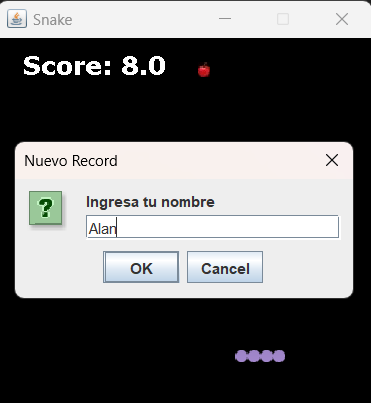
\includegraphics[width=0.4\textwidth]{P2.png}
    \end{figure}
    
    \item Vea el episodio 4 de la serie IA y de su opinión al respecto: \url{https://youtu.be/Kr1fmKVY3cA?list=PLjq6DwYksrzz_fsWIpPcf6V7p2RNAneKc}
    
    La exploración de la inteligencia artificial (I.A.) genera interrogantes intrigantes acerca de sus fronteras y aplicaciones. Desde replicar atributos humanos hasta la participación de máquinas en deportes y cine, se despliega un panorama amplio y estimulante. La iniciativa de diseñar muñecos realistas y emplear I.A. en relaciones personales suscita cuestionamientos éticos.

    Roborace destaca el desafío de crear autos autónomos capaces de superar las habilidades humanas en carreras. La competencia entre equipos resalta la complejidad de desarrollar I.A. segura y eficiente. El extracto de Superman y Lois Lane agrega un toque de humor y reflexión sobre las percepciones de las limitaciones de la I.A.

    La información refleja el continuo debate en torno a los límites de la I.A. y sus repercusiones en diversos aspectos de la vida diaria, desde las relaciones personales hasta las competiciones de alto nivel. La amalgama de avances tecnológicos y desafíos éticos plantea interrogantes cruciales sobre el futuro de la I.A. en nuestra sociedad.

    \item Estudie el tema de \textit{Externalizable} ubicado en: \url{https://www.geeksforgeeks.org/externalizable-interface-java/}
    
    Explique cual serian las diferencias con \textit{Serializable} con sus propias palabras.

    La principal disparidad entre \textit{Serializable} y \textit{Externalizable} en Java radica en cómo gestionan la serialización de objetos.

    \textit{Serializable} simplifica la serialización al llevar a cabo este proceso de forma automática, eliminando la necesidad de especificar qué campos deben ser serializados. Al implementar la interfaz, los objetos pueden ser serializados sin complicaciones.

    Externalizable demanda que el programador implemente dos métodos: \textit{writeExternal} y \textit{readExternal}.

    Mientras \textit{Serializable} emplea el método de serialización predeterminado proporcionado por Java, \textit{Externalizable} permite personalizar el proceso, determinando qué datos deben escribirse y en qué formato.
  \end{enumerate}

  \section*{Referencias}
  \textit{Externalizable interface in Java.} (2017, October 16). GeeksforGeeks; GeeksforGeeks. \url{https://www.geeksforgeeks.org/externalizable-interface-java/} \\

  \textit{POO/TemaVI.ManejoArchivos/Principal.java at main · LeonardoLed/POO.} (2023). GitHub. \url{https://github.com/LeonardoLed/POO/blob/main/TemaVI.ManejoArchivos/Principal.java} \\

  YouTube Originals. (2019, December 18). \textit{Love, art and stories: decoded | The Age of A.I.} [Video]. YouTube. \url{https://www.youtube.com/watch?v=Kr1fmKVY3cA}
\end{document}